% =====================================================================
%  Dense scientific report — source document for a MICCAI workshop paper
%  Topic: reliability of segmentation evaluation under imperfect GT
%  Build:  pdflatex main.tex  (x2 for refs)  — no external bib tool needed
%  NOTE:   sections marked %% PENDING await the running experiments (Q1/Q2/Q3).
% =====================================================================
\documentclass[11pt,a4paper]{article}

\usepackage[utf8]{inputenc}
\usepackage[T1]{fontenc}
\usepackage[margin=2.4cm]{geometry}
\usepackage{amsmath,amssymb,amsthm}
\usepackage{graphicx}
\usepackage{booktabs}
\usepackage{xcolor}
\usepackage{enumitem}
\usepackage{caption}
\usepackage{subcaption}
\usepackage[hidelinks]{hyperref}
\usepackage{microtype}

\graphicspath{{figures/}}

\newcommand{\gtstar}{\ensuremath{\mathrm{GT}^{\!*}}}
\newcommand{\gtminus}{\ensuremath{\mathrm{GT}^{\!-}}}
\newcommand{\Nop}{\ensuremath{\mathcal{N}}}
\newcommand{\R}{\ensuremath{\mathbb{R}}}
\newcommand{\E}{\ensuremath{\mathbb{E}}}
\newcommand{\todo}[1]{{\color{red}\textbf{[TODO: #1]}}}

\title{\textbf{On the Reliability of Segmentation Model Evaluation\\
under Imperfect Ground Truth:\\
A Formal Annotation--Noise Model and an Ethical Inquiry}}
\author{M.\ Codjia}
\date{\today}

\begin{document}
\maketitle

\begin{abstract}
Deep-learning segmentation models are trained \emph{and evaluated} against manual
annotations that are themselves imperfect: inter-observer disagreement on tubular
structures such as pulmonary vessels is well documented. We ask a question that is
usually left implicit: \emph{if the reference is noisy, are our model rankings
trustworthy?} We introduce a formal, calibrated annotation-noise operator
$\gtminus = \Nop(\gtstar;\theta)$ parametrised by a family, a scale $r$, a severity
$p$, a directional bias $\mu$, and a seed. The operator unifies, under a single
knob $\mu$, the literature's central distinction between \emph{unbiased} noise
(zero-mean boundary jitter, which behaves as augmentation) and \emph{biased} noise
(systematic over/under-segmentation, which can be learned). Using this instrument we
formalise three questions on the PARSE pulmonary-artery dataset with nnU-Net: (Q1)
does evaluating on $\gtminus$ unfairly penalise a clean-trained model? (Q2) does
unbiased label noise act as data augmentation? (Q3) can a systematic annotation bias
be \emph{learned}, making a model fit the wrong reference better? A recurring finding
is metrological: the matched metric must agree with the noise not only in
\emph{type} (topological vs.\ surface) but in \emph{scale} and \emph{direction}; we
show that a clinically realistic boundary error is below the resolving power of
standard surface metrics, and that on thin vessels surface and topological errors are
inseparable. We argue these observations carry an ethical weight for how the
community reports and trusts evaluation.
\end{abstract}

% =====================================================================
\section{Introduction}
% =====================================================================
Supervised image segmentation rests on a silent assumption: that the manual
annotation used as ground truth (\gtstar) is correct. In practice annotations are
produced by humans under time pressure, vary between observers, and are especially
unreliable on thin, branching structures where a one-voxel disagreement on the vessel
wall is a large fraction of the lumen. The same imperfect annotations are used to
\emph{train} models and, more consequentially, to \emph{evaluate} and \emph{rank}
them. When a benchmark declares model~$A$ better than model~$B$ by a small margin on
a metric computed against a noisy reference, we rarely ask whether that ranking
survives the noise.

This report makes that question explicit and tractable. We do not study a new
architecture; we study the \emph{measurement apparatus} of segmentation research --
the annotation and the metric -- and the conditions under which it produces
trustworthy verdicts. Our contributions are:
\begin{enumerate}[leftmargin=1.4em,itemsep=2pt]
  \item A \textbf{formal annotation-noise operator} $\Nop(\gtstar;\theta)$ with a
  small, interpretable parameter vector $\theta$, calibrated to an inter-observer
  agreement (IAA) window measured on real data (Sec.~\ref{sec:formalism}).
  \item A single continuous \textbf{bias parameter $\mu$} that interpolates between
  unbiased jitter (augmentation regime) and systematic, learnable bias, unifying the
  biased/unbiased dichotomy of the literature (Sec.~\ref{sec:formalism}).
  \item Three \textbf{pre-registered research questions} (Q1--Q3) with an explicit
  \emph{instrument-matching} methodology that pairs each noise with the metric
  sensitive to it in type, scale and direction (Sec.~\ref{sec:methodology}).
  \item A set of \textbf{metrological observations} -- realistic boundary error is
  sub-clinical for standard metrics; surface and topology are inseparable on thin
  vessels -- with direct \textbf{ethical implications} for evaluation practice
  (Sec.~\ref{sec:ethics}).
\end{enumerate}

% =====================================================================
\section{Related Work}\label{sec:related}
% =====================================================================
\paragraph{Imperfect labels.} Heller et al.~\cite{heller2018imperfect} systematically
perturbed segmentation labels and reported the counter-intuitive result that networks
are remarkably robust to \emph{unbiased}, zero-mean boundary noise -- displacements
cancel across slices and the model recovers the mean boundary -- whereas
\emph{systematic} biases (consistent under-segmentation, omissions) genuinely degrade
performance. Our $\mu$ parameter is a direct operationalisation of this dichotomy.

\paragraph{Boundary perturbation models.} Simple morphological erosion/dilation is
spatially uniform and structurally unrealistic. Markov-process boundary perturbations
\cite{yao2023markov} and the GSD-Net line~\cite{gsdnet2025} distort contours
irregularly and allow a foreground-reducing ($S_R$) or foreground-expanding ($S_E$)
bias; our \texttt{boundary\_drift} family follows this idea with a smoothed
correlated displacement field plus a constant drift.

\paragraph{Topology-aware metrics.} clDice~\cite{shit2021cldice} measures the overlap
of morphological \emph{skeletons} and is the standard for tubular connectivity; by
construction it is insensitive to boundary displacement -- a fact that becomes central
to our instrument-matching argument.

\paragraph{Framework and data.} We use nnU-Net~\cite{isensee2021nnunet} on the
PARSE pulmonary-artery dataset~\cite{parse2022}. Surface agreement is quantified with
the Normalised Surface Dice (NSD)~\cite{nikolov2018nsd} and the 95th-percentile
Hausdorff distance (HD95).

% =====================================================================
\section{Formalism}\label{sec:formalism}
% =====================================================================
\subsection{The annotation-noise operator}
Let $\gtstar\subseteq\Omega$ be a clean binary annotation on a voxel grid $\Omega$
with anisotropic spacing $s=(s_1,s_2,s_3)$ mm. A degraded annotation is the image of a
stochastic operator
\begin{equation}
  \gtminus \;=\; \Nop(\gtstar;\theta),
  \qquad
  \theta=(\varphi,\,r,\,p,\,\mu,\,\text{seed}),
\end{equation}
where $\varphi$ selects a \emph{family} (mechanism), $r$ is a \emph{scale}
(radius/amplitude/length), $p$ a \emph{severity} (fraction or per-unit probability),
$\mu$ a \emph{directional bias} (boundary family only), and the seed fixes the random
realisation, making $\Nop$ reproducible to the voxel. \textbf{Application policy:}
$\Nop$ is applied to \emph{every} image (and every training batch); $p$ is never a
probability of applying the operator, only a severity. Code-level guarantees ensure at
least one structural unit or surface voxel is affected whenever $p>0$.

\subsection{Families}
We use two complementary mechanisms (a third, \texttt{distal\_truncation}, is
discarded as redundant with omission; see Sec.~\ref{sec:calib}).

\paragraph{Topological: \texttt{distal\_omission}.} A morphological opening
$\gamma_r=\delta_r\!\circ\!\varepsilon_r$ with a ball of radius $r$ removes every
structure thinner than $r$. The removable set is partitioned into connected
components, each deleted independently with probability $p$:
\begin{equation}
  \gtminus \;=\; \gtstar \;\setminus\!\!\bigcup_{c\,:\,b_c=1}\!\! C_c,
  \qquad C_c\subseteq \gtstar\setminus\gamma_r(\gtstar),
  \quad b_c\sim\text{Bernoulli}(p).
\end{equation}
This is a \emph{biased}, foreground-reducing, topology-altering noise: it deletes
distal branches.

\paragraph{Surface/directional: \texttt{boundary\_drift}.} Let
$\phi(x)$ be the signed distance to $\partial\gtstar$ ($\phi<0$ inside). The boundary
is displaced by a field combining a constant drift and a smoothed zero-mean
fluctuation $\xi$ of correlation length $\ell$:
\begin{equation}
  d(x) \;=\; a\,\big(\mu + \xi(x)\big)\,g_p(x),
  \qquad a = r\,\bar{s},\quad \E[\xi]=0,
  \label{eq:drift}
\end{equation}
\begin{equation}
  \gtminus \;=\; \{\,x:\ \phi(x)-d(x)\le 0\,\},
\end{equation}
where $\bar s$ is the mean spacing and $g_p$ a surface coverage gate selecting a
fraction $p$ of boundary voxels. Equation~\eqref{eq:drift} \textbf{decomposes the
boundary error into a systematic and a stochastic part}:
\begin{equation}
  \underbrace{a\,\mu\,g_p}_{\text{systematic, \emph{learnable}}}
  \;+\;
  \underbrace{a\,\xi\,g_p}_{\text{zero-mean, \emph{augmentation}}}.
\end{equation}

\subsection{The bias axis $\mu$}
The single parameter $\mu$ indexes the entire experimental axis
(Fig.~\ref{fig:musweep}):
\[
  \mu<0:\ \text{under-segmentation (eroded boundary)};\quad
  \mu=0:\ \text{pure jitter};\quad
  \mu>0:\ \text{over-segmentation}.
\]
A noise is \emph{unbiased} iff $\E[\Delta V]=0$, where
$\Delta V=(|\gtminus|-|\gtstar|)/|\gtstar|$ is the signed relative volume change. For
$\mu=0$ the zero-mean fluctuation averages out across resampled realisations and acts
as augmentation; for $\mu\neq0$ the systematic component is constant across
realisations and can be \emph{learned}. This is the formal bridge between the noise
parametrisation and the research questions of Sec.~\ref{sec:methodology}.

\begin{figure}[t]
  \centering
  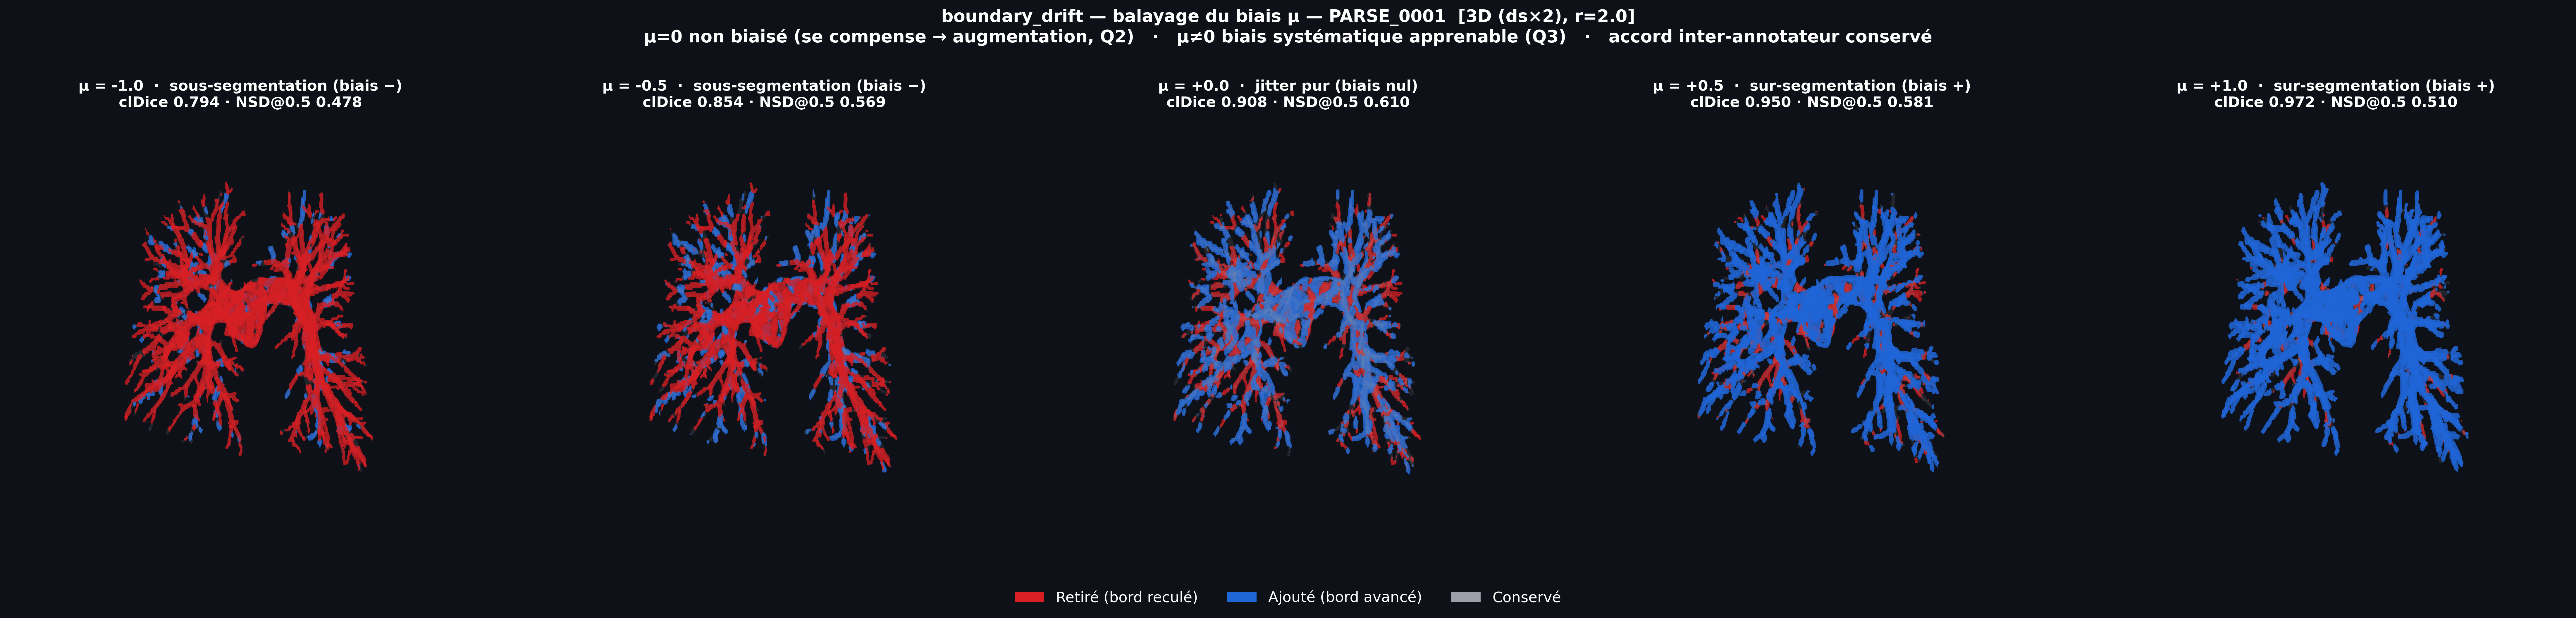
\includegraphics[width=\linewidth]{drift_mu_sweep_3d_PARSE_0001.png}
  \caption{\textbf{The bias axis $\mu$ on a real pulmonary-artery tree.} Red = removed
  voxels (boundary receded), blue = added (boundary advanced). From left to right
  $\mu=-1,\,-0.5,\,0,\,+0.5,\,+1$: under-segmentation $\to$ balanced jitter $\to$
  over-segmentation. The inter-annotator agreement (clDice, NSD@0.5\,mm) is annotated
  under each view, showing the operating range stays realistic. A single parameter
  spans augmentation ($\mu=0$, Q2) and learnable bias ($\mu\neq0$, Q3).}
  \label{fig:musweep}
\end{figure}

\begin{figure}[t]
  \centering
  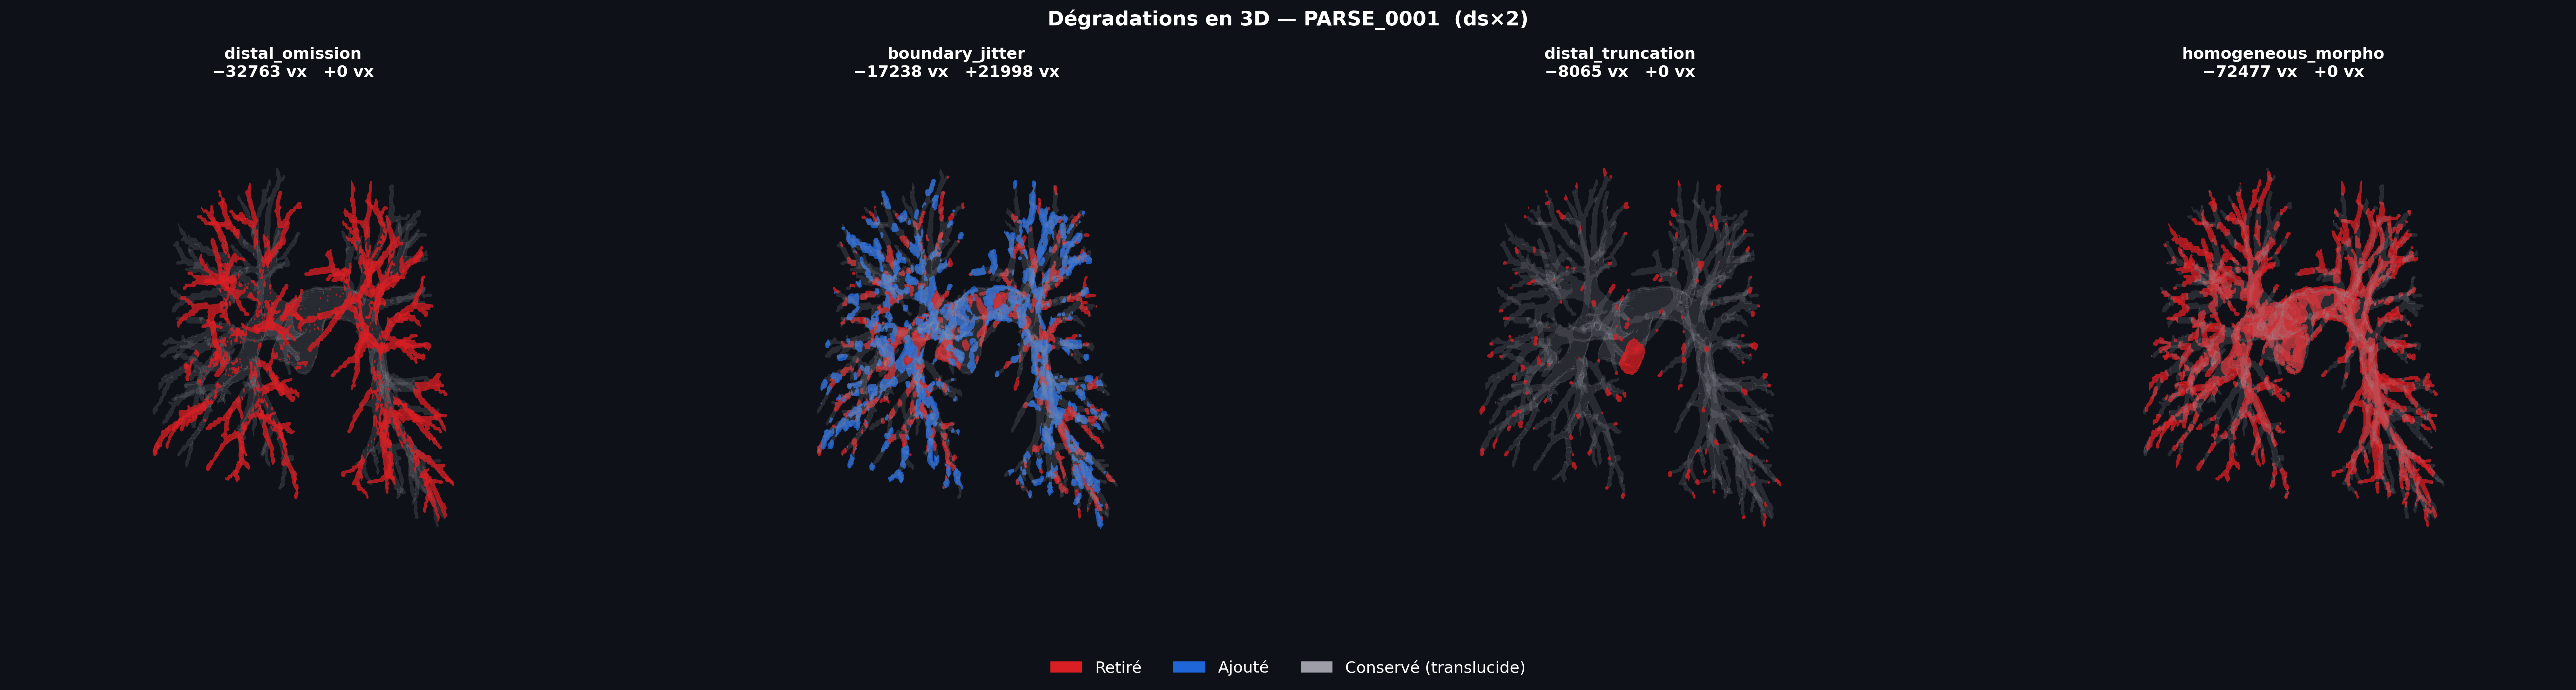
\includegraphics[width=\linewidth]{degradation_3d_PARSE_0001.png}
  \caption{\textbf{Signatures of the noise families} (3D). Voxel counts in the titles
  expose the bias: \texttt{distal\_omission}, \texttt{distal\_truncation} and
  \texttt{homogeneous\_morpho} only remove ($-N/+0$, biased), whereas
  \texttt{boundary\_drift} at $\mu=0$ removes and adds in near-equal amounts
  (unbiased) -- the visual fingerprint of zero-mean noise (cf.~Heller et
  al.~\cite{heller2018imperfect}).}
  \label{fig:families}
\end{figure}

% =====================================================================
\section{Methodology}\label{sec:methodology}
% =====================================================================
\subsection{Guiding principles}
\textbf{(i) One family at a time.} We never compose noises until each is understood in
isolation; this removes hard-to-debug confounds and gives clean causal attribution.
\textbf{(ii) Match the instrument to the quantity} -- in type, scale \emph{and}
direction (Table~\ref{tab:pairing}). \textbf{(iii) The biased/unbiased axis} organises
the questions: biased noise penalises (Q1) and is learnable (Q3); unbiased noise is
benign and augments (Q2).

\begin{table}[t]
  \centering
  \caption{Instrument--noise pairing. The off-axis (witness) metric should stay flat;
  for the drift, surface and topology are coupled on thin vessels (Sec.~\ref{sec:coupling}).}
  \label{tab:pairing}
  \small
  \begin{tabular}{lll}
    \toprule
    Noise & Primary instrument & Rationale \\
    \midrule
    \texttt{distal\_omission} (topological) & clDice, Betti$_0$ & connectivity / branch deletion \\
    \texttt{boundary\_drift} magnitude & NSD@0.5\,mm & sub-voxel surface displacement \\
    \texttt{boundary\_drift} direction ($\mu$) & signed $\Delta V$ & NSD/HD95 are unsigned \\
    \bottomrule
  \end{tabular}
\end{table}

\subsection{Calibration to inter-observer agreement}\label{sec:calib}
Operating points are \emph{measured}, not assumed, on PARSE via
\texttt{calibrate\_noise.py}, targeting $\text{clDice}(\gtminus,\gtstar)\in[0.85,0.90]$:
\texttt{distal\_omission} $r{=}2,p{=}0.3\to$ clDice $0.878$; \texttt{boundary\_drift}
$r{=}1,p{=}0.5\to$ NSD@0.5 $\approx 0.88$. \texttt{distal\_truncation} is discarded
because it is \emph{redundant} with omission (same biased, distal foreground-reduction
axis); its high clDice is not evidence of harmlessness but of a \emph{mismatched
instrument} -- clDice cannot see edge filing.

\subsection{Models and training regimes}
A shared clean baseline plus one model per condition
(Table~\ref{tab:models}). The training regime is dictated by the question, not chosen
arbitrarily:
\begin{itemize}[leftmargin=1.4em,itemsep=2pt]
  \item \textbf{On-the-fly} (fresh realisation each epoch) for Q2: augmentation
  \emph{is} resampling; a frozen $\mu{=}0$ set would teach the frozen ripple, not
  robustness.
  \item \textbf{Fixed} (one realisation per case) for Q3: a cohort of annotators is a
  single, consistent realisation; a stable biased target is what a model can learn,
  without the augmentation confound. This is the realistic scenario.
\end{itemize}

\begin{table}[t]
  \centering
  \caption{Experimental matrix (nnU-Net, $500$ epochs).}
  \label{tab:models}
  \small
  \begin{tabular}{llll}
    \toprule
    Model & Trained on & Regime & Serves \\
    \midrule
    $M_0$ Star          & $\gtstar$ (clean)                 & standard    & baseline \\
    $M_1$ Omission      & \texttt{distal\_omission} $r2\,p0.3$ & on-the-fly & Q1, Q2 \\
    $M_2$ Drift $\mu{=}0$  & \texttt{boundary\_drift} $r1\,p0.5\,\mu0$ & on-the-fly & Q2 \\
    $M_3$ Drift $\mu{<}0$  & \texttt{boundary\_drift} $\mu{=}{-}0.5$ (fixed) & fixed & Q3 \\
    $M_4$ Drift $\mu{>}0$  & \texttt{boundary\_drift} $\mu{=}{+}0.5$ (fixed) & fixed & Q3 \\
    \bottomrule
  \end{tabular}
\end{table}

\subsection{Research questions}
For a metric $m$ (higher better), a model $M$, and a reference $R\in\{\gtstar,\gtminus\}$,
write $m(M\mid R)$ for the per-case score; all tests are paired Wilcoxon signed-rank
($n{=}15$) with paired Cohen's $d$, and report the minimum detectable difference (MDD)
when non-significant.

\paragraph{Q1 -- Artificial penalty.} $M_0$ is evaluated against $\gtstar$ and against
$\gtminus$; \emph{only the reference changes}. A significant drop
$m(M_0\mid\gtstar)\!>\!m(M_0\mid\gtminus)$ implicates the GT, not the model.
Matched metric: clDice/Betti$_0$ for omission, $\Delta V$/NSD for drift.

\paragraph{Q2 -- Robustness / augmentation.} $M_2$ (unbiased, on-the-fly) vs.\ $M_0$,
\emph{both evaluated on clean $\gtstar$}. $\mu{=}0$ isolates robustness: with no bias
to match, any benefit is regularisation. Hypothesis $m(M_2\mid\gtstar)\ge m(M_0\mid\gtstar)$.

\paragraph{Q3 -- Learned bias.} $M_3$ (biased, fixed) evaluated against the biased
$\gtminus$ and against $\gtstar$. If the bias is learned, the penalty on the biased
reference is \emph{smaller} than for $M_0$, while the deviation from $\gtstar$ is
\emph{larger} ($\Delta V(M_3)<0$): the model fits the wrong data better.

\subsection{The thin-vessel coupling}\label{sec:coupling}
On sub-millimetre tubular structures, surface and topological errors are not
separable: a boundary displacement comparable to the vessel radius pinches the vessel.
We verified (26-connectivity, $N(\gtstar){=}1$) that \texttt{boundary\_drift} genuinely
fragments the tree ($N\approx59$ at $r1\,p0.5$). This is not an artefact but a real
property of annotation error on thin structures, and it bounds what any ``surface-only''
study can claim.

% =====================================================================
\section{Results}\label{sec:results}
% =====================================================================
\subsection{Noise calibration (acquired)}
%% The calibration table is final; reproduce from results/noise_calibration.csv.
Table of operating points and the dissociation evidence
(clDice insensitive to drift; NSD@0.5 insensitive to $\mu$ direction; HD95 saturated)
is reported in Sec.~\ref{sec:calib} and Fig.~\ref{fig:musweep}.

\subsection{Q1 / Q2 / Q3 (pending experiments)}
%% PENDING: fill from results/ once orchestrator.py --tiers AB completes.
\todo{Insert paired-Wilcoxon tables (clDice, Betti$_0$, NSD@0.5, $\Delta V$), effect
sizes and MDDs for Q1--Q3; per-model boxplots across scenarios.}

% =====================================================================
\section{Discussion}\label{sec:discussion}
% =====================================================================
\paragraph{A metrological motivation.} For $\mu{=}0$ we expect the model-to-model
difference to be small, possibly below metric sensitivity. We therefore cannot
distinguish ``no effect'' from ``effect below resolution''. This is precisely why the
\emph{sensitivity} of the metrics themselves (their minimum detectable difference) must
be studied alongside the models -- a measurement cannot be trusted beyond the
resolution of its instrument.

\paragraph{Which noise mis-ranks models.} Our design predicts that biased noise
(omission, drift $\mu\neq0$) both penalises and is learnable, while unbiased boundary
jitter is largely benign. The practical corollary is that the dangerous annotation
errors for benchmarking are the \emph{systematic} ones -- exactly the ones a single
annotator or a single labelling protocol is most likely to introduce.

% =====================================================================
\section{Ethical Inquiry}\label{sec:ethics}
% =====================================================================
The technical results above are, at root, an ethical argument about how the community
produces and trusts evidence.

\paragraph{Rankings under noisy references may not be real.} If a systematic
annotation bias shifts a metric by more than the gap between two models, the published
ranking reflects the annotator, not the algorithm. Deploying the ``winner'' is then a
decision made on a measurement artefact -- with clinical consequences downstream.

\paragraph{Annotation quality is an ethical responsibility, not a logistics detail.}
The biased/unbiased dichotomy gives this a sharp form: a lab can tolerate
\emph{random} labelling noise (it averages out) but must guard against \emph{systematic}
protocol bias, which both inflates apparent performance on its own data and can be
silently learned by the model.

\paragraph{Recommendations for evaluation practice.}
\begin{enumerate}[leftmargin=1.4em,itemsep=2pt]
  \item Report the \emph{inter-observer agreement} of the reference and the metric's
  minimum detectable difference; treat any model gap below the MDD as undecided.
  \item Match the metric to the failure mode being claimed (type, scale, direction);
  do not infer harmlessness from a metric blind to the perturbation.
  \item Prefer \emph{multi-annotator} or bias-audited references for any benchmark used
  to select a model for clinical use.
\end{enumerate}

% =====================================================================
\section{Conclusion}
% =====================================================================
We framed annotation noise as a formal, calibrated operator with a single bias axis,
turned three intuitive questions into pre-registered, instrument-matched tests, and
surfaced metrological limits -- realistic boundary error is sub-clinical for standard
metrics, and surface and topology are inseparable on thin vessels. Beyond the numbers
(forthcoming), the work is a plea for measurement humility in segmentation: a model is
only as trustworthy as the reference and the metric we judge it by.

% =====================================================================
\begin{thebibliography}{9}
\small
\bibitem{heller2018imperfect} N.~Heller, J.~Dean, N.~Papanikolopoulos.
  \emph{Imperfect Segmentation Labels: How Much Do They Matter?} MICCAI LABELS
  workshop, 2018.
\bibitem{yao2023markov} \todo{Yao et al., 2023 -- Markov-process boundary perturbation;
  verify exact title/venue.}
\bibitem{gsdnet2025} \todo{GSD-Net, 2025 -- boundary-aware label-noise robust
  segmentation; verify reference.}
\bibitem{shit2021cldice} S.~Shit et al. \emph{clDice -- a Novel Topology-Preserving
  Loss Function for Tubular Structure Segmentation.} CVPR, 2021.
\bibitem{isensee2021nnunet} F.~Isensee et al. \emph{nnU-Net: a self-configuring method
  for deep learning-based biomedical image segmentation.} Nature Methods, 2021.
\bibitem{parse2022} \todo{PARSE 2022 challenge -- pulmonary artery segmentation;
  verify citation.}
\bibitem{nikolov2018nsd} S.~Nikolov et al. \emph{Deep learning to achieve clinically
  applicable segmentation of head and neck anatomy (Normalised Surface Dice).}
  arXiv:1809.04430, 2018.
\end{thebibliography}

\end{document}
